%standard 14.3

%start_of_questions



%new_question
%%%%%%%%%%%%%%%%%%%%%
	% Problem 13
	% Difficulty: 3
%%%%%%%%%%%%%%%%%%%%%
	\item 
		Create a python program that writes the name and age of everyone in your family to .csv file.
		There should be a column for the name with a header titled Name, and there should be a column 
		for the age with a header titled Age.
		Do not use the csv module. You may make up fake family members if you choose. The result
		should look similar to the following.
		
		\begin{flushright}
			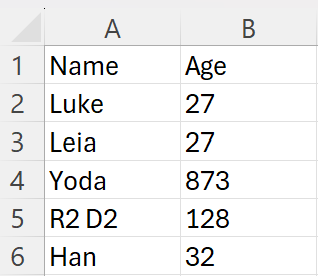
\includegraphics[scale=.65]{imgs/WritingFamily.PNG}
		\end{flushright}



%Write a few that write to write with multiple columns using a clear delimeter. 



%end_of_questions
%make sure to leave at least one blank line below

